
\documentclass[xcolor={usenames,dvipsnames},12pt,presentation,aspectratio=169]{beamer}

\usepackage[utf8]{inputenc}
\usepackage{fontawesome}
\usepackage[brazilian]{babel}
\usepackage{verbatim}
\usepackage{graphicx}
\usepackage{xspace}
\usepackage{amsthm}
\usepackage{url}
\usepackage{array}
\usepackage{hyperref}
\usepackage{times,mathptmx}
\usepackage{pdfpages}
\usepackage{mdframed}
\usepackage{tikz}
\usepackage{alltt}
\usepackage{minted}
%\usepackage{times}
%\usepackage[usenames,dvipsnames]{xcolor}
%\usepackage[usenames,dvipsnames]{color}
%\usepackage{color}

\usetikzlibrary{arrows,shapes}

\usetheme{Madrid}
%\usetheme{Boadilla}
%\usetheme{Darmstadt}
%\usetheme{Frankfurt}
%\usetheme{CambridgeUS}
%\usetheme{AnnArbor}
%\usecolortheme{beaver}
%\usecolortheme{seahorse}
%\usecolortheme{seagull}
\usecolortheme[named=BrickRed]{structure}

\setbeamercovered{transparent}

\setbeamertemplate{footline}[frame number]
%\setbeamertemplate{navigation symbols}{}
%\setbeamersize{text margin left=1em,text margin right=1em}

\newcommand{\titulo}{Programação Paralela com MPI}
\newcommand{\disciplina}{ELC139 - Programação Paralela}
\newcommand{\nome}{João Vicente Ferreira Lima (UFSM)}

\lecture[1]{\aula}{aula01}
\def\lecturename{\aula}

\newcommand{\Red}[1]{{\color{red}#1}}
\newcommand{\red}[1]{{\color{red}#1}}
\newcommand{\Blue}[1]{{\color{blue}#1}}
\newcommand{\blue}[1]{{\color{blue}#1}}

\newcommand{\PBS}[1]{\let\temp=\\#1\let\\=\temp}
\newcommand{\RRCOL}{\PBS\raggedright\hspace{0pt}}

\newcommand{\p}[1]{\texttt{#1}}
\newenvironment{code}{%
  \begin{alltt}%
  }{%
  \end{alltt}%
}

\makeatletter
%\setbeamertemplate{headline}{}
% {%
%   \leavevmode%
%   \@tempdimb=2.4375ex%
%   \ifnum\beamer@subsectionmax<\beamer@sectionmax%
%     \multiply\@tempdimb by 4%
%   \else%
%     \multiply\@tempdimb by\beamer@subsectionmax%
%   \fi%
%   \ifdim\@tempdimb>0pt%
%     \advance\@tempdimb by 1.125ex%
%     \begin{beamercolorbox}[wd=.5\paperwidth,ht=\@tempdimb]{section in head/foot}%
%       \vbox to\@tempdimb{\vfil\insertsectionnavigation{.5\paperwidth}\vfil}%
%     \end{beamercolorbox}%
%     \begin{beamercolorbox}[wd=.45\paperwidth,ht=\@tempdimb]{subsection in head/foot}%
%       \vbox
%       to\@tempdimb{\vfil\insertsubsectionnavigation{.45\paperwidth}\vfil}%
%     \end{beamercolorbox}%
%     \begin{beamercolorbox}[wd=.05\paperwidth,ht=\@tempdimb]{subsection in head/foot}%
%       \vbox
%       to\@tempdimb{\vfil\hfil\insertframenumber\vfil\vfil}%
%     \end{beamercolorbox}%
%   \fi%
% }

\def\dohead{\beamer@headcounter=4\relax\beamer@headcounter=1\loop\ifnum\beamer@headcounter<\beamer@totalheads%
  \advance\beamer@headcounter by1\relax%
  \csname @@head\the\beamer@headcounter\endcsname\repeat}

\makeatother

\title[\titulo]{\titulo}

\subtitle{\disciplina}

\author[João V. F. Lima]{\nome}

%\institute[UFSM]{Departamento de Linguagens e Sistemas de Computação \\ Universidade Federal de Santa Maria \\ \url{jvlima@inf.ufsm.br} \\ \url{http://www.inf.ufsm.br/~jvlima}}
\institute[UFSM]{Universidade Federal de Santa Maria \\ \url{jvlima@inf.ufsm.br} \\ \url{http://www.inf.ufsm.br/~jvlima}}
\date{2023/1}

\graphicspath{{.}{figs/}}

\logo{ 
\includegraphics[height=1.5cm,width=1.5cm,keepaspectratio]{logo_inf}    
        
\includegraphics[height=1.5cm,width=1.5cm,keepaspectratio]{logo_ufsm} }

%\titlegraphic{
%	
\includegraphics[width=2cm]{logo_ufsm}
%  \hspace{1cm}
%	
\includegraphics[width=2cm]{logo_inf}
%}

\newtheorem{mydef}{Definição}[section]
%\newtheorem{myteo}{Teorema}[section]
%------------------------------------------------------------------------------
%\newcommand{\xkaapi}{XKaapi\xspace}
%------------------------------------------------------------------------------
% Typesetting Listings
\usepackage{listings}
\lstset{
  language=C,
  %basicstyle=\scriptsize\ttfamily,
  %basicstyle=\normalsize\ttfamily,
  basicstyle=\small\ttfamily,
  %basicstyle=\footnotesize\ttfamily,
  %aboveskip=0pt,
  %belowskip=0pt,
  %mathescape=false,
  columns=fullflexible,
  %numbers=none,
  numbers=left,
  numbersep=5pt,
%  showtabs=true,
%  showspaces=true,
  frame=tb,
  breaklines=true
}
%------------------------------------------------------------------------------
%\lstset{commentstyle=\color{blue}}
%\lstset{stringstyle=\ttfamily}
%\lstset{ classoffset=1, 
%            morekeywords={kaapi,omp,task,data,alloca, declare, reduction, identity, parallel,sync,taskwait,cilk,spawn,tbb,css,cilk\_spawn,cilk\_sync,cilk\_for,offload},
%            keywordstyle=\color{Red}\bfseries
%           }
%\lstset{ classoffset=2, 
%            morekeywords={value,read,write,readwrite,reduction,untied,firstprivate,TaskBodyCPU,TaskBodyGPU,ka,Signature,RW,CW,range2d\_r,range2d\_rw,range2d,Spawn,Fork,Shared\_w,Shared\_r,Shared,a1,target,device,copyin,copyout,input,implements,copy\_deps,RPWP,range2d\_rpwp,rangeindex,Memory,Register,SetStaticSched,Sync,Unregister,Community,System,join\_community,SpawnMain,leave,initialize,terminate,logfile,array,SetArch,ArchHost,ArchCUDA,W,R,gpuStream,pointer\_w,pointer\_r,pointer\_cw,pointer},
%            keywordstyle=\color{Blue}\bfseries
%           }
%\lstset{ classoffset=3, 
%            morekeywords={storage,ld},
%            keywordstyle=\bfseries
%           }
%\lstset{ classoffset=4, 
%            morekeywords={in,out,inout,cout,concurrent},
%            keywordstyle=\color{Red}\bfseries
%           }
%           
%\lstset{classoffset=0, showstringspaces=false}
%------------------------------------------------------------------------------
\mdfsetup{
  backgroundcolor=gray!10,
%  roundcorner=10pt,
}
%------------------------------------------------------------------------------
\newcommand{\restorefootline}{\setbeamertemplate{navigation symbols}{}}
%\newcommand{\setfootline}[1]{\setbeamertemplate{navigation symbols}{\textcolor{black}{\textbf{#1}}}}
\newcommand{\includeslides}[4]{%
%  \setfootline{#1}%
  {
    \setbeamercolor{background canvas}{bg=}
    \includepdf[pages={#1},%
    pagecommand={},
%    pagecommand={\begin{frame}[default]{}\end{frame}},
%    #4,%
    turn=false,noautoscale=false,column=false,columnstrict=false,openright=false,frame=false]{#2}%
  }
  %\restorefootline%
}
%------------------------------------------------------------------------------
\begin{document}

\begin{frame}
%  \titlepage
  \maketitle
%  \mode<presentation>
%  {
%    \begin{columns}
%      \begin{column}{0.5\textwidth}
%      \raggedleft
%	
\includegraphics[width=2cm]{logo_ufsm}
%      \end{column}
%      \begin{column}{0.5\textwidth}
%	
\includegraphics[width=2cm]{logo_inf}
%      \end{column}
%    \end{columns}
%  }
\end{frame}

\begin{frame}
    \frametitle{Outline}
%    \tableofcontents[hideallsubsections]
    \tableofcontents
\end{frame}

\AtBeginSection{
  \begin{frame}
    \frametitle{Outline}
    \tableofcontents[currentsection]
  \end{frame}
}

\AtBeginSubsection[]
{
    \begin{frame}
        \frametitle{Outline}
        \tableofcontents[currentsection,currentsubsection]
    \end{frame}
}

%%%%%%%%%%%%%%%%%%%%%%%%%%%%%%%%%%%%%%%%%%%%%%%%%%%%%%%%%%%%%%%%%%%%%%%%%%%%%%
\section{Comunicações coletivas}
%%%%%%%%%%%%%%%%%%%%%%%%%%%%%%%%%%%%%%%%%%%%%%%%%%%%%%%%%%%%%%%%%%%%%%%%%%%%%%%
%------------------------------------------------------------------------------
\begin{frame}[fragile]
  \frametitle{Comunicações coletivas}
  \begin{itemize}
    \item O que poderia melhorar com relação a versão vista anteriormente?
  \end{itemize}
\begin{center}
\begin{minipage}{0.95\textwidth}
  \begin{minted}[linenos, fontsize=\small, breaklines=true, frame=lines]{C}
/* Input: a, b, n */
h = (b - a)/n;
approx = (f(a) + f(b))/2.0;
for (i = 1; i <= n - 1; i++) {
  x i = a + i*h;
  approx += f(x i);
}
approx = h*approx;
  \end{minted}
\end{minipage}
\end{center}
\end{frame}
%------------------------------------------------------------------------------
\begin{frame}[fragile]
  \frametitle{Aproximação trapezoidal com MPI}
\begin{center}
\begin{minipage}{0.95\textwidth}
  \begin{minted}[linenos, fontsize=\small, breaklines=true, frame=lines]{C}
  /* Add up the integrals calculated by each process */
  if (my_rank != 0) { 
      MPI_Send(&local_int, 1, MPI_DOUBLE, 0, 0, 
            MPI_COMM_WORLD); 
  } else {
      total_int = local_int;
      for (source = 1; source < comm_sz; source++) {
        MPI_Recv(&local_int, 1, MPI_DOUBLE, source, 0,
            MPI_COMM_WORLD, MPI_STATUS_IGNORE);
        total_int += local_int;
      }
  } 
  \end{minted}
\end{minipage}
\end{center}
\end{frame}
%------------------------------------------------------------------------------
\begin{frame}[fragile]
  \frametitle{Comunicações coletivas}
  \begin{itemize}
    \item Processo mestre faz todo o trabalho de soma!!
    \item Como distribuir esse trabalho entre os processos?
  \end{itemize}
\begin{center}
\begin{minipage}{0.95\textwidth}
  \begin{minted}[linenos, fontsize=\small, breaklines=true, frame=lines]{C}
/* Input: a, b, n */
h = (b - a)/n;
approx = (f(a) + f(b))/2.0;
for (i = 1; i <= n - 1; i++) {
  x i = a + i*h;
  approx += f(x i);
}
approx = h*approx;
  \end{minted}
\end{minipage}
\end{center}
\end{frame}
%------------------------------------------------------------------------------
\begin{frame}
  \frametitle{Soma estruturada em árvore}
  \vspace{-3mm}
  \begin{center}
	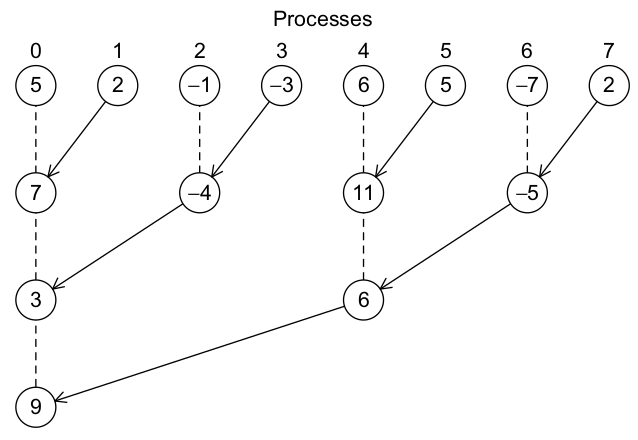
\includegraphics[width=0.6\textwidth]{col1.png}
  \end{center}
  \vspace{-4mm}
  {\tiny An Introduction to Parallel Programming, Peter Pacheco, 2011.}
\end{frame}
%------------------------------------------------------------------------------
\begin{frame}
  \frametitle{Soma estruturada em árvore}
  \vspace{-3mm}
  \begin{center}
	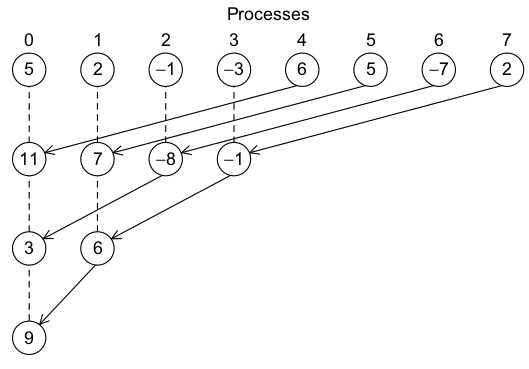
\includegraphics[width=0.6\textwidth]{col2.png}
  \end{center}
  \vspace{-4mm}
  {\tiny An Introduction to Parallel Programming, Peter Pacheco, 2011.}
\end{frame}
%------------------------------------------------------------------------------
\begin{frame}[fragile]
  \frametitle{Aproximação trapezoidal com MPI}
  Uma versão com comunicação coletiva.
\begin{center}
\begin{minipage}{0.95\textwidth}
  \begin{minted}[linenos, fontsize=\small, breaklines=true, frame=lines]{C}
    MPI_Reduce( &local_int, &total_int, 
      1, MPI_DOUBLE, 
      MPI_SUM, 
      0, MPI_COMM_WORLD );
  \end{minted}
\end{minipage}
\end{center}
\end{frame}
%------------------------------------------------------------------------------
\begin{frame}
  \frametitle{Comunicações coletivas}
  \begin{itemize}
    \item Todos os processos precisam chamar a mesma função coletiva no mesmo comunicador.
    \item Os argumentos precisam ser compatíveis. Se um processo coloca como destino $0$ e outro $1$, o programa trava ou aborta.
    \item O(s) parâmetro(s) de saída são usados apenas no processo destino.
    \item As comunicações ponto-a-ponto usam tags e comunicadores como Identificador. Por outro lado, comunicações coletivas usam apenas o comunicador e \emph{ordem} de execução.
  \end{itemize}
\end{frame}
%%%%%%%%%%%%%%%%%%%%%%%%%%%%%%%%%%%%%%%%%%%%%%%%%%%%%%%%%%%%%%%%%%%%%%%%%%%%%%
\subsection{Allreduce}
%%%%%%%%%%%%%%%%%%%%%%%%%%%%%%%%%%%%%%%%%%%%%%%%%%%%%%%%%%%%%%%%%%%%%%%%%%%%%%%
%------------------------------------------------------------------------------
\begin{frame}[fragile]
  \frametitle{\mintinline{C}{MPI_Allreduce}}
  Quando todos os processos precisam do resultado.
\begin{center}
\begin{minipage}{0.95\textwidth}
  \begin{minted}[linenos, fontsize=\small, breaklines=true, frame=lines]{C}
int MPI_Allreduce(
  const void *sendbuf,      /* in */
  void *recvbuf,            /* out */
  int count,                /* in */
  MPI_Datatype datatype,    /* in */
  MPI_Op op,                /* in */
  MPI_Comm comm             /* in */
)
  \end{minted}
\end{minipage}
\end{center}
\end{frame}
%------------------------------------------------------------------------------
\begin{frame}
  \frametitle{\mintinline{C}{MPI_Allreduce}}
  \vspace{-3mm}
  \begin{center}
	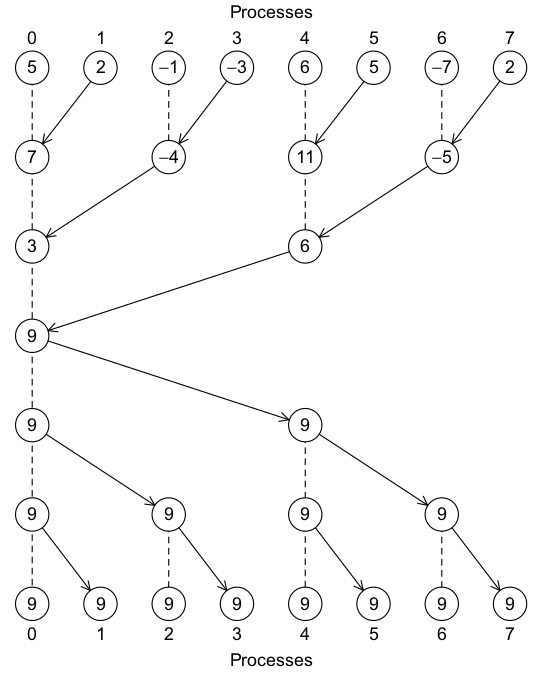
\includegraphics[width=0.4\textwidth]{allreduce1.png}
  \end{center}
  \vspace{-4mm}
  {\tiny An Introduction to Parallel Programming, Peter Pacheco, 2011.}
\end{frame}
%------------------------------------------------------------------------------
\begin{frame}
  \frametitle{\mintinline{C}{MPI_Allreduce}}
  \vspace{-3mm}
  \begin{center}
	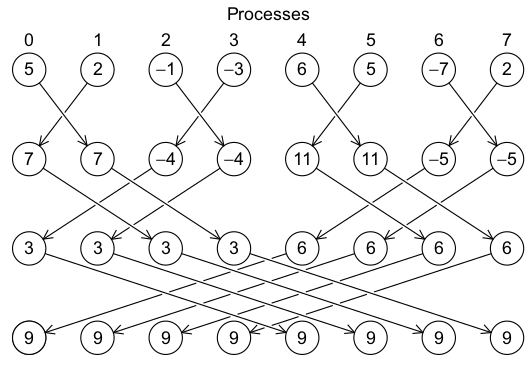
\includegraphics[width=0.6\textwidth]{allreduce2.png}
  \end{center}
  \vspace{-4mm}
  {\tiny An Introduction to Parallel Programming, Peter Pacheco, 2011.}
\end{frame}
%%%%%%%%%%%%%%%%%%%%%%%%%%%%%%%%%%%%%%%%%%%%%%%%%%%%%%%%%%%%%%%%%%%%%%%%%%%%%%
\subsection{Broadcast}
%%%%%%%%%%%%%%%%%%%%%%%%%%%%%%%%%%%%%%%%%%%%%%%%%%%%%%%%%%%%%%%%%%%%%%%%%%%%%%%
%------------------------------------------------------------------------------
\begin{frame}[fragile]
  \frametitle{Broadcast}
  Dados de um processo são enviados a todos os outros do comunicador.
\begin{center}
\begin{minipage}{0.95\textwidth}
  \begin{minted}[linenos, fontsize=\small, breaklines=true, frame=lines]{C}
int MPI_Bcast( 
    void *buffer,
    int count,
    MPI_Datatype datatype,
    int root, 
    MPI_Comm comm
  )
  \end{minted}
\end{minipage}
\end{center}
\end{frame}
%------------------------------------------------------------------------------
\begin{frame}
  \frametitle{Broadcast}
  \vspace{-3mm}
  \begin{center}
	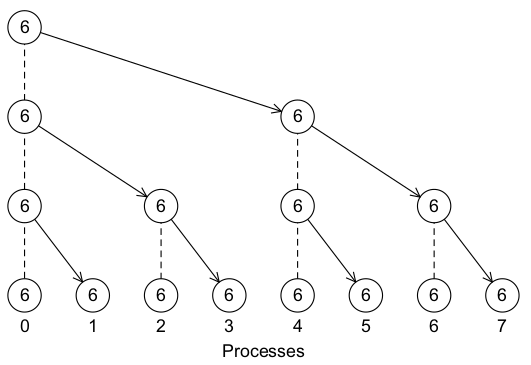
\includegraphics[width=0.6\textwidth]{bcast.png}
  \end{center}
  \vspace{-4mm}
  {\tiny An Introduction to Parallel Programming, Peter Pacheco, 2011.}
\end{frame}
%%%%%%%%%%%%%%%%%%%%%%%%%%%%%%%%%%%%%%%%%%%%%%%%%%%%%%%%%%%%%%%%%%%%%%%%%%%%%%
\subsection{Scatter}
%%%%%%%%%%%%%%%%%%%%%%%%%%%%%%%%%%%%%%%%%%%%%%%%%%%%%%%%%%%%%%%%%%%%%%%%%%%%%%%
%------------------------------------------------------------------------------
\begin{frame}[fragile]
  \frametitle{Soma vetorial}
  Podemos usar broadcast de vetores?
\begin{center}
\begin{minipage}{0.95\textwidth}
  \begin{minted}[linenos, fontsize=\small, breaklines=true, frame=lines]{C}
void Parallel_vector_sum(
      double  local_x[]  /* in  */, 
      double  local_y[]  /* in  */, 
      double  local_z[]  /* out */, 
      int     local_n    /* in  */) {
   int local_i;

   for (local_i = 0; local_i < local_n; local_i++)
      local_z[local_i] = local_x[local_i] + local_y[local_i];
}  /* Parallel_vector_sum */

  \end{minted}
\end{minipage}
\end{center}
\end{frame}
%------------------------------------------------------------------------------
\begin{frame}[fragile]
  \frametitle{Scatter}
Scatter divide os dados entre os processos e envia um pedaço para cada processo.
\begin{columns}
  \begin{column}{0.5\textwidth} 
    \begin{center}
      \begin{minipage}{0.95\textwidth}
        \begin{minted}[linenos, fontsize=\small, breaklines=true, frame=lines]{C}
int MPI_Scatter(
    const void *sendbuf,
    int sendcount,
    MPI_Datatype sendtype,
    void *recvbuf,
    int recvcount,
    MPI_Datatype recvtype,
    int root,
    MPI_Comm comm
)
        \end{minted}
      \end{minipage}
      \end{center}    
  \end{column}
  \begin{column}{0.5\textwidth}
    \begin{center}
    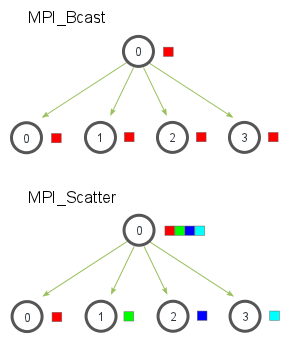
\includegraphics[width=0.6\textwidth]{broadcastvsscatter.png}
    \end{center}       
  \end{column}
\end{columns}
{\tiny https://mpitutorial.com/tutorials/mpi-scatter-gather-and-allgather/}
\end{frame}
%------------------------------------------------------------------------------
\begin{frame}[fragile]
  \frametitle{Soma vetorial}
Scatter divide os dados entre os processos e envia um pedaço para cada processo.
\begin{center}
\begin{minipage}{0.95\textwidth}
  \begin{minted}[linenos, fontsize=\small, breaklines=true, frame=lines]{C}
if (my_rank == 0) {
  /* lê dados de algum lugar */
  MPI_Scatter(a, local_n, MPI_DOUBLE, local_a, local_n, 
    MPI_DOUBLE, 0, comm);
} else {
  MPI_Scatter(a, local_n, MPI_DOUBLE, local_a, local_n,
    MPI_DOUBLE, 0, comm);
}
  \end{minted}
\end{minipage}
\end{center}
\end{frame}
%%%%%%%%%%%%%%%%%%%%%%%%%%%%%%%%%%%%%%%%%%%%%%%%%%%%%%%%%%%%%%%%%%%%%%%%%%%%%%
\subsection{Gather}
%%%%%%%%%%%%%%%%%%%%%%%%%%%%%%%%%%%%%%%%%%%%%%%%%%%%%%%%%%%%%%%%%%%%%%%%%%%%%%%
%------------------------------------------------------------------------------
\begin{frame}[fragile]
  \frametitle{Gather}
Gather coleta dados de todos os processos e agrupa.
\begin{columns}
  \begin{column}{0.5\textwidth}
    \begin{center}
      \begin{minipage}{0.95\textwidth}
        \begin{minted}[linenos, fontsize=\small, breaklines=true, frame=lines]{C}
int MPI_Gather(
  const void *sendbuf,
  int sendcount,
  MPI_Datatype sendtype,
  void *recvbuf,
  int recvcount,
  MPI_Datatype recvtype,
  int root,
  MPI_Comm comm
)
        \end{minted}
      \end{minipage}
      \end{center}    
  \end{column}
  \begin{column}{0.5\textwidth}
    \begin{center}
    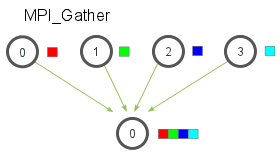
\includegraphics[width=\textwidth]{gather.png}
    \end{center}       
  \end{column}
\end{columns}
{\tiny https://mpitutorial.com/tutorials/mpi-scatter-gather-and-allgather/}
\end{frame}
%------------------------------------------------------------------------------
\begin{frame}[fragile]
  \frametitle{Soma vetorial}
  Gather coleta dados de todos os processos e agrupa.
\begin{center}
\begin{minipage}{0.95\textwidth}
  \begin{minted}[linenos, fontsize=\small, breaklines=true, frame=lines]{C}
if (my_rank == 0) {
  MPI_Gather(local_b, local_n, MPI_DOUBLE, b, local_n,
    MPI_DOUBLE, 0, comm);
} else {
  MPI_Gather(local_b, local_n, MPI_DOUBLE, b, local_n,
    MPI_DOUBLE, 0, comm);
}
  \end{minted}
\end{minipage}
\end{center}
\end{frame}
%%%%%%%%%%%%%%%%%%%%%%%%%%%%%%%%%%%%%%%%%%%%%%%%%%%%%%%%%%%%%%%%%%%%%%%%%%%%%%
\subsection{Allgather}
%%%%%%%%%%%%%%%%%%%%%%%%%%%%%%%%%%%%%%%%%%%%%%%%%%%%%%%%%%%%%%%%%%%%%%%%%%%%%%%
%------------------------------------------------------------------------------
\begin{frame}[fragile]
  \frametitle{Allgather}
  Multiplicação vetor matriz -- $y = Ax$
\begin{center}
\begin{minipage}{0.95\textwidth}
  \begin{minted}[linenos, fontsize=\small, breaklines=true, frame=lines]{C}
for (i = 0; i < m; i++) {
  y[i] = 0.0;
  for (j = 0; j < n; j++)
    y[i] += A[i][j]*x[j];
  }
  \end{minted}
\end{minipage}
\end{center}
\end{frame}
%------------------------------------------------------------------------------
\begin{frame}[fragile]
  \frametitle{Allgather}
  Multiplicação vetor matriz -- $y = Ax$
  \begin{center}
    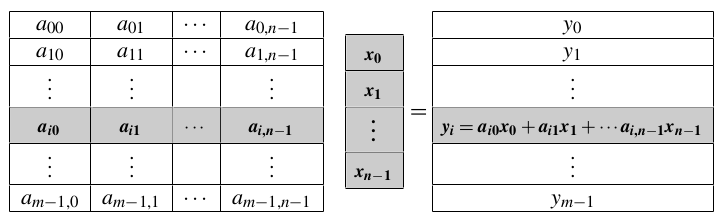
\includegraphics[width=\textwidth]{matrix-vector.png}
    \end{center}      
\end{frame}
%------------------------------------------------------------------------------
\begin{frame}[fragile]
  \frametitle{Allgather}
\begin{center}
\begin{minipage}{0.95\textwidth}
  \begin{minted}[linenos, fontsize=\small, breaklines=true, frame=lines]{C}
void Mat_vect_mult(
      double  A[]  /* in  */, 
      double  x[]  /* in  */, 
      double  y[]  /* out */,
      int     m    /* in  */, 
      int     n    /* in  */) {
  int i, j;

  for (i = 0; i < m; i++) {
    y[i] = 0.0;
    for (j = 0; j < n; j++)
      y[i] += A[i*n+j]*x[j];
    }
  }  /* Mat_vect_mult */
  \end{minted}
\end{minipage}
\end{center}
\end{frame}
%------------------------------------------------------------------------------
\begin{frame}[fragile]
  \frametitle{Allgather}
Agrupa dados de todos os processos e faz \emph{broadcast}.
\begin{columns}
  \begin{column}{0.5\textwidth}
    \begin{center}
      \begin{minipage}{0.95\textwidth}
        \begin{minted}[linenos, fontsize=\small, breaklines=true, frame=lines]{C}
int MPI_Allgather(
  const void *sendbuf,
  int sendcount,
  MPI_Datatype sendtype,
  void *recvbuf,
  int recvcount,
  MPI_Datatype recvtype,
  MPI_Comm comm
)
        \end{minted}
      \end{minipage}
      \end{center}    
  \end{column}
  \begin{column}{0.5\textwidth}
    \begin{center}
    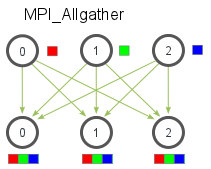
\includegraphics[width=0.9\textwidth]{allgather.png}
    \end{center}       
  \end{column}
\end{columns}
{\tiny https://mpitutorial.com/tutorials/mpi-scatter-gather-and-allgather/}
\end{frame}
%------------------------------------------------------------------------------
\begin{frame}[fragile]
  \frametitle{Allgather}
\begin{center}
\begin{minipage}{0.95\textwidth}
  \begin{minted}[linenos, fontsize=\small, breaklines=true, frame=lines]{C}
double* x;
int local_i, j;
int local_ok = 1;

x = malloc(n*sizeof(double));
MPI_Allgather(local_x, local_n, MPI_DOUBLE,
      x, local_n, MPI_DOUBLE, comm);

for (local_i = 0; local_i < local_m; local_i++) {
  local_y[local_i] = 0.0;
  for (j = 0; j < n; j++)
      local_y[local_i] += local_A[local_i*n+j]*x[j];
}
free(x);  
  \end{minted}
\end{minipage}
\end{center}
\end{frame}
%------------------------------------------------------------------------------
\begin{frame}[plain]{}
  \begin{center}
    \vspace{2cm}
    \Large{https://joao-ufsm.github.io/par2023a/}
    
    \vspace{1cm}
    
\includegraphics[width=2cm]{logo_ufsm}
    \hspace{0.5cm}
    
\includegraphics[width=2cm]{logo_inf}
  \end{center}
\end{frame}
%------------------------------------------------------------------------------

\end{document}
